%!TEX root = ../crimson_throne_book_main.tex
% 2015-10-24
When darkness has fallen over the city, Neolandus Kalepopolis leads the party to the Great Tower, the headquarters of his order, the Sable Company, and home of their magnificent flying mounts, the hippogriffs. Officially there are only two ways into this massive tower, the front gate on the third floor and the flying platform in the aerie, 250 feet off the ground. Fortunately, the seneschal knows a third way in: a secret door in the back. Upon whispering the words "For safety in the air and on the water" the outline of a hippogriff head lights up in the palm of his hand. When he touches it to the cool stone, a secret door slides open. A small set of stairs takes the heroes to the second floor of the Tower, where a gruesome scene awaits them: the bodies of three dead Sable Marines. Neolandus swallows down his disgust and shows the others to the central staircase, which takes them directly to the entry hall on the third floor.\hyperref[fig:Gray-Maidens-in-the-Great-Tower-567993387]{ Eleven Gray Maidens are guarding the front doors here and they are quite surprised to see people emerging from } Quint casts  {\itshape haste} on his companions and starts  {\itshape satire} , warning the warrior women to stand down or perish. Up to this point, none of the heroes has ever crossed swords with the queen's elite soldiers, and the bard would prefer to avoid a bloody confrontation. His words do not impress the armor-clad maidens, though, and their commander orders her troops to attack. The Gray Maidens seem to work well together, strengthening each other's attacks and defenses. Balian is surrounded and takes several hits. Puk, Vencarlo and Spyder try to hold the line, giving Quint the opportunity to use  {\itshape pyrotechnics} on the fire in the hearth. The fireplace blazes up in a flash of light, blinding over half of the opponents. Sjo follows up with a mighty fireball, which burns badly through the female knights. Blinded and scorched, the Gray Maidens fall quickly to the companions' blades. When Sjo summons a second fiery explosion, the fight is as good as over. The remaining warrior women die in the last seconds of hand-to hand combat. \\

\begin{figure}[h]
	\centering
	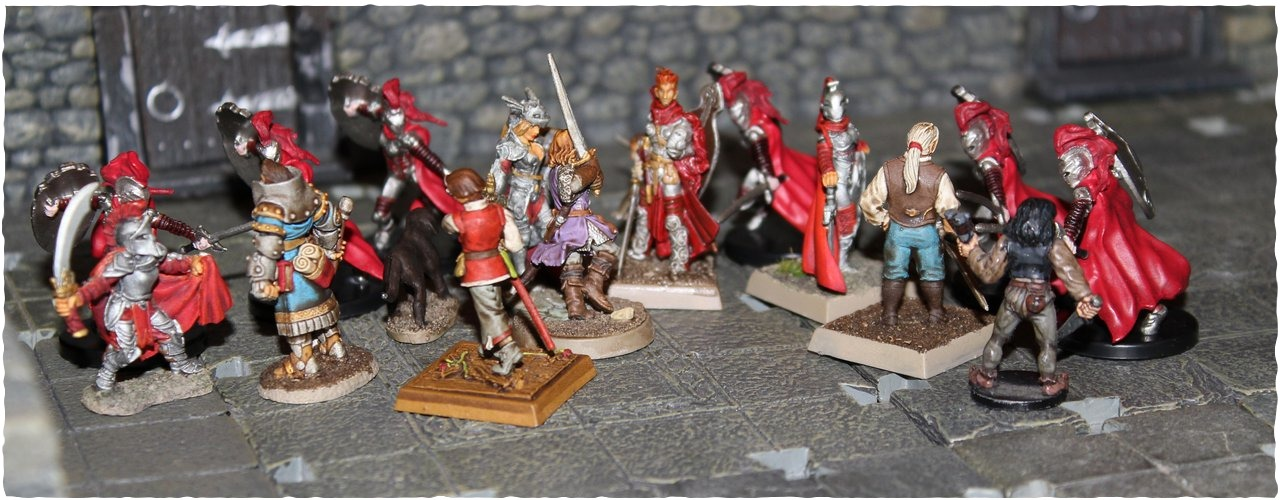
\includegraphics[width=0.4\textwidth]{images/Gray-Maidens-in-the-Great-Tower-567993387_mod.jpg}
	\caption{Gray Maidens in the Great Tower}
	\label{fig:Gray-Maidens-in-the-Great-Tower-567993387}
\end{figure}

The companions continue their way up. On the fourth floor they discover more bodies of slain Sable Marines. While Kalepopolis closes their eyes and wishes them well on their way to whatever paradise they deserve, Quint slips into the chapel of Iomedae, where he prays to the goddess of valor and justice for forgiveness for his aid in ending the lives of the Gray Maidens downstairs. On the next floor Neolandus Kalepopolis still has his personal quarters. He opens a secret cache in the wall, from which he pulls weapons and armor. His new attire is very ostentatious, a vibrantly red silk vest with puffy shoulders and a similar pair of pants. He also dons a red wide-brimmed hat with a flowing peacock feather and a matching cloak. "If we're going to fight the power, we might as well do it in style", he smiles. "Now, let's go up and free the hippogriffs!"\\

\hyperref[fig:Great-Tower-stables-in-Korvosa-567993978]{ The stables start on the fifteenth floor. } Sjo knows this place well, as he used to work here for a time, hoping to become a Sable Marine himself. His impaired vision quickly spoiled these aspirations, though. The stables reek badly, as if they haven't been cleaned properly in a few days. The snorts of unhappy hippogriffs from behind closed doors tell the companions that the animals are still alive, just like they had hoped. Two half-orcs guard this floor, but seeing a group of well-armed and battle-ready heroes burst into the room has them flee up the stairs, calling out for someone named 'Grenk'. Quint recalls hearing about a cruel half-orc beast master who went by that name. Our friends find this character on the top floor, the aerie, \hyperref[fig:Korvosa-Great-Tower-Aerie-567995366]{ where he and some minions are viciously trying to tame a couple of hippogriffs. } The brute draws his axe, bellows out a  {\itshape terrifying howl} which sends Puk and Spyder running in fear. This is the only success he manages in the fight, though, for the beast master and his goons are quickly overrun. Vencarlo shows his skill with the rapier and stabs down two of Grenk's helps, while Quint's  {\itshape cacophonous call} takes away the half-orc leader's ability to fight. The raging brute makes for the platform, hoping to crawl away over the walls with his  {\itshape slippers of spider climbing} , but he never makes it. Quint trips him as Balian unleashes greatsword hell on his ass. Before Grenk can get up again, Sjo freezes him in place with a  {\itshape hold person} . The party shows the cruel animal trainer no mercy. \\

\begin{figure}[h]
	\centering
	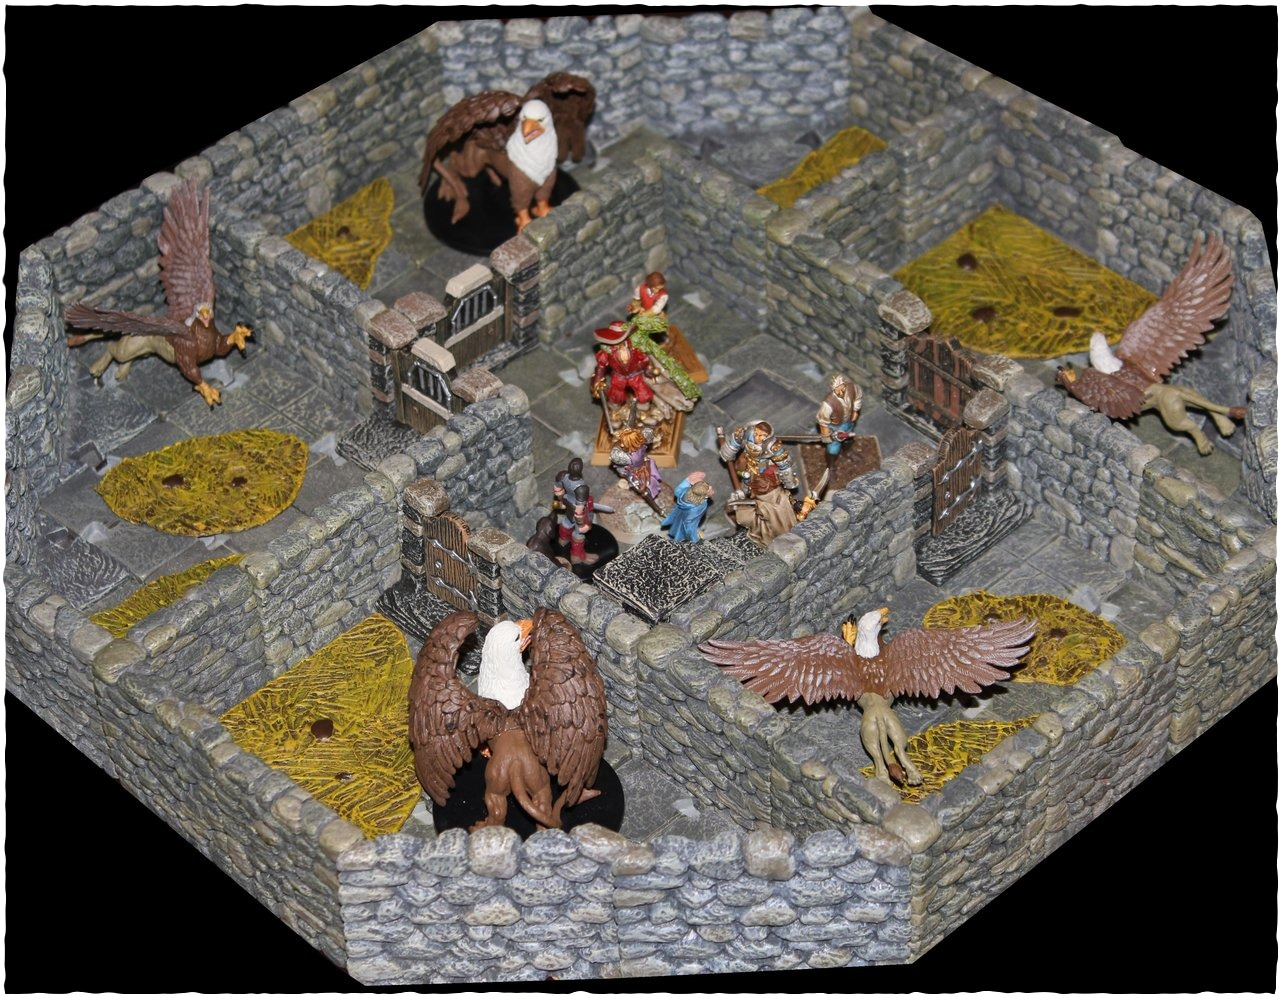
\includegraphics[width=0.4\textwidth]{images/Great-Tower-stables-in-Korvosa-567993978_mod.jpg}
	\caption{Great Tower stables in Korvosa}
	\label{fig:Great-Tower-stables-in-Korvosa-567993978}
\end{figure}

\begin{figure}[h]
	\centering
	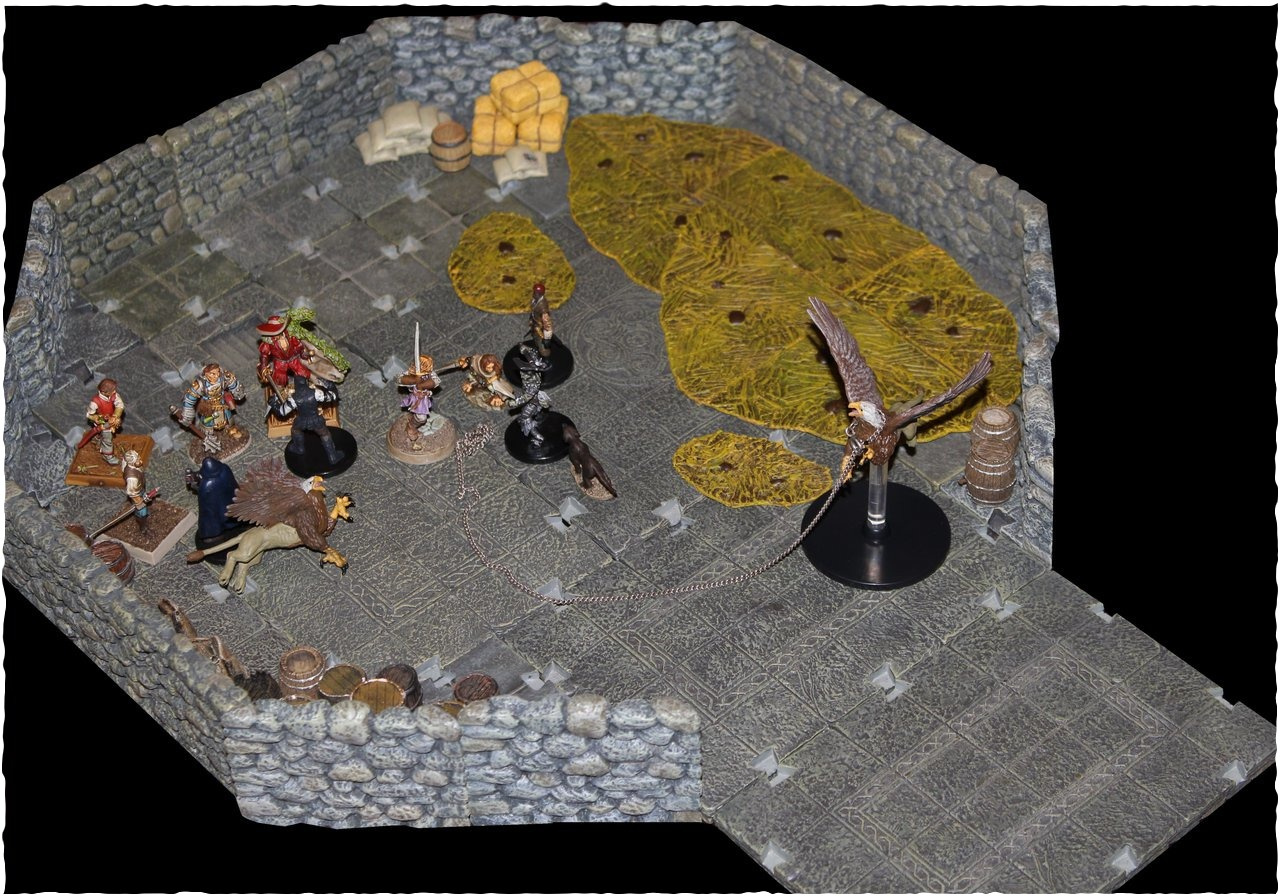
\includegraphics[width=0.4\textwidth]{images/Korvosa-Great-Tower-Aerie-567995366_mod.jpg}
	\caption{Korvosa Great Tower Aerie}
	\label{fig:Korvosa-Great-Tower-Aerie-567995366}
\end{figure}

Neolandus Kalepopolis and Sjo show the others how to saddle the hippogriffs and lead all the animals upstairs. The seneschal designates each companions a mount, before sending the remaining hippogriffs into the air.\hyperref[fig:Freeing-the-Sable-Company-mounts-567995944]{ "Fly, my pretties, fly!" } he proudly shouts. "Don't worry about them, or your own mount, either," Kalepopolis tells the party. "All of them will follow my steed, Silverback. Just hang on tight and make sure you don't fall. Tie yourselves down if you have to. And most of all: ENJOY!" At that he orders his gray-backed winged stallion off the platform and into the air. \\

\begin{figure}[h]
	\centering
	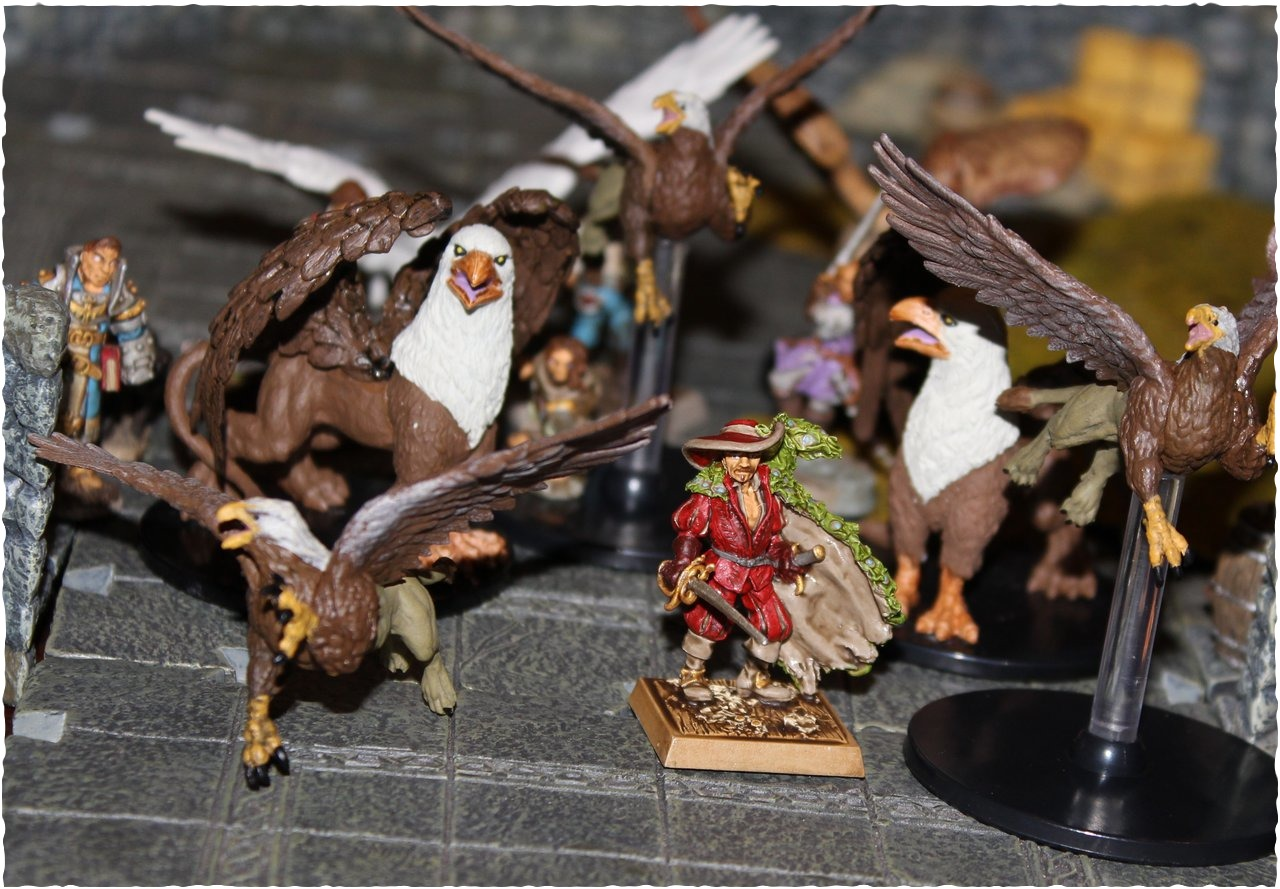
\includegraphics[width=0.4\textwidth]{images/Freeing-the-Sable-Company-mounts-567995944_mod.jpg}
	\caption{Freeing the Sable Company mounts}
	\label{fig:Freeing-the-Sable-Company-mounts-567995944}
\end{figure}

